\documentclass{article}
\usepackage{graphicx} % Required for inserting images
\usepackage{hyperref}
\usepackage{tikz}
\usepackage{tabularray}
\usepackage{pgfplots}
\usepackage{float}

\title{Optimization of Numerical Benchmark Functions Using the Genetic Algorithm}
\author{Denis Crismariu}
\date{\today}
\begin{document}

\maketitle

\abstract
This report investigates the application of Genetic Algorithms (GA) for optimizing mathematical functions. The study focuses on the implementation and experimentation with different fitness evaluation functions to enhance the performance of the GA. Through detailed experimentation, we evaluate the efficiency and accuracy of the GA on four benchmark functions: De Jong’s, Schwefel’s, Rastrigin’s, and Michalewicz’s comparing it to our previous results using Hill Climb and Simulated Annealing. This report aims to provide insights into the effectiveness of various fitness evaluation strategies and encoding methods in genetic algorithms and suggests potential areas for further research and improvement.


\section{Introduction}
This report details the use of Genetic Algorithms (GA) for optimizing mathematical functions and compares the results with Hill Climbing algorithms. The study focuses on the implementation and experimentation with different fitness evaluation functions to enhance the performance of the GA. Specifically, our objective is to search for the minima of four benchmark functions: De Jong’s, Schwefel’s, Rastrigin’s, and Michalewicz’s.

The GA starts with an initial population of potential solutions, represented as binary strings. Each generation involves fitness evaluation, selection, crossover, and mutation. 

Hill Climbing algorithms, including First Improvement and Best Improvement variants, are also employed for comparison. The First Improvement variant quickly accepts the first neighboring solution that improves the objective function, making it faster but potentially less accurate. The Best Improvement variant evaluates all neighboring solutions and selects the best one, generally leading to better solutions but at the cost of increased computational time.

This report aims to provide a detailed analysis of the GA's performance on the benchmark functions, highlighting the impact of different fitness evaluation strategies and encoding methods. By comparing their performance with Hill Climbing algorithms, we seek to understand the trade-offs involved and explore potential strategies for enhancing the algorithms' performance. The findings of this study could inform the development of more robust optimization techniques for a wide range of applications.
Our experiments show that the Genetic Algorithm is, on average, 6653\% faster but 8\% less accurate compared to the Best Improvement version of the Hill Climbing algorithm.



\section{Methods \& Implementation}
The implementation of a Genetic Algorithm (GA) involves setting parameters that influence its efficiency. We set the population size to 100, the mutation probability of $\frac{1}{L}$ and 1000 generations. Additionally, we set the precision to be $10^{-5}$ and the dimensions to 5, 10, and 30.

Our approach to the GA follows a distinct order: fitness evaluation, selection, crossover and mutation.

Each generation concludes with the fitness evaluation of the new population. The fitness of each individual is calculated based on the objective function we aim to minimize. We experimented with different fitness evaluation functions to enhance the performance of the genetic algorithm. For instance: \\
$f' = \left(\frac{(max - f)}{(max - min + \epsilon)} + 1\right)^2$ for Schwefel and Rastrigin, $f'=\frac{1}{f+\epsilon}$ for De Jong and $f' = \left(\frac{(max - f)}{(max - min + \epsilon)} + 1\right)^3$ for Michalewicz.

The selection and crossover process takes place next. In this phase, two parents are selected based on roulette wheel selection. Each chromosome from the parents has a 50\% chance of being passed to the offspring, creating two new offspring that inherit a blend of genetic material from both parents. Additionally, the best individual from the current generation is copied directly to the next generation to ensure that the highest fitness solution is preserved.

The mutation step, applied to the newly created individuals with the best from the last generation as an exception, introduces random changes in the genetic makeup of the individuals. This process, governed by the mutation probability, is vital for injecting new genetic traits into the population, thereby enhancing its diversity and aiding in the exploration of new areas in the solution space. This is done by flipping the bits in the binary strings at a probability set in the initial phase.



\section{Experimental results}
The 4 benchmarked functions are the following:
\newpage
\subsection{Rastrigin Function\cite{Rastrigin}}

$$ f(x) = A \cdot n + \sum_{i=1}^n \left[ x_i^2 - A \cdot cos(2 \pi x_i) \right],
A = 10, x_i \in \left[ -5.12, 5.15 \right]$$

The global minima is located at $f(x)=0; x(i)=0,  \forall i=1:n $
\begin{figure}[!h]
  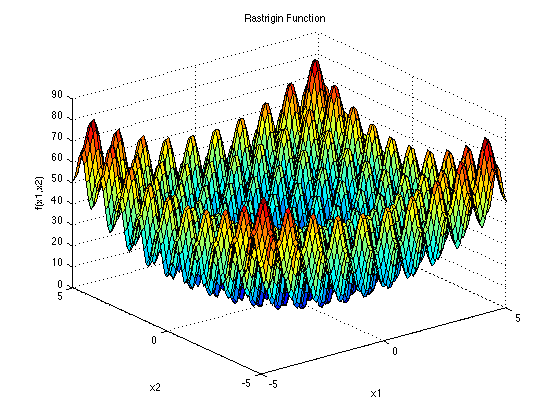
\includegraphics[width=\textwidth,height=\textheight,keepaspectratio]{rastr.png}
  \caption{Rastrigin Function\cite{rast_img}}
\end{figure}
\begin{table}[H]
\caption{Values based on 30 runs}
\begin{tblr}{
colspec={X[0.96,l] X[1.7,l] X[1,l] X[1,l] X[1,l] X[1,l]},
rowsep=0.01pt,  % Reduce the vertical padding between cell contents and borders
  cell{1}{1} = {c=2}{},
  cell{2}{1} = {r=4}{c},
  cell{6}{1} = {r=4}{c},
  cell{10}{1} = {r=4}{c},
  vlines,
  hline{1-2,6,10,14} = {-}{},
  hline{3-5,7-9,11-13} = {2-7}{},
}
     &              & HC Best & HC  First & HC Worst & SA Best & GA\\
D = 5 & Mean error & 0.994 & 0.994 & 0.000 & 0.000 & 0.001 \\
      &   SDev error & 0.505 & 0.530 & 0.495 & 0.495 & 0.005 \\
      &   Min error & 0.000 & 0.000 & 0.000 & 0.000 & 0.000 \\
      &   Max error & 1.000 & 1.994 & 1.000 & 0.995 & 0.031 \\

D = 10 & Mean error & 4.346 & 5.456 & 4.225 & 4.343 & 3.935 \\
     &   SDev error & 0.857 & 1.030 & 1.060 & 1.130 & 2.148 \\
     &   Min error & 2.235 & 4.220 & 1.994 & 1.995 & 1.040 \\
     &   Max error & 5.984 & 7.692 & 5.466 & 6.225 & 9.419 \\

D = 30 & Mean error & 28.516 & 36.637 & 29.511 & 30.881 & 31.982 \\
     &   SDev error & 2.509 & 2.680 & 3.466 & 2.509 & 6.757 \\
     &   Min error & 20.789 & 31.226 & 19.897 & 24.593 & 19.837 \\
     &   Max error & 31.904 & 39.687 & 32.836 & 34.739 & 46.042 \\
\end{tblr}
\caption{Hill Climbing time (in seconds) based on 30 runs}
\begin{tblr}{
colspec={X[0.96,l] X[1.7,l] X[1,l] X[1,l] X[1,l] X[1,l]},
rowsep=0.01pt,  % Reduce the vertical padding between cell contents and borders
  cell{1}{1} = {c=2}{},
  cell{2}{1} = {r=4}{c},
  cell{6}{1} = {r=4}{c},
  cell{10}{1} = {r=4}{c},
  vlines,
  hline{1-2,6,10,14} = {-}{},
  hline{3-5,7-9,11-13} = {2-7}{},
}
     &              & HC Best & HC  First & HC Worst & SA Best & GA \\
D = 5 & Mean time & 0.794 & 0.495 & 0.647 & 4.772 & 0.207 \\
     &   SDev time & 0.016 & 0.002 & 0.008 & 0.012 & 0.005 \\
     &   Min time & 0.767 & 0.491 & 0.635 & 4.753 & 0.205 \\
     &   Max time & 0.838 & 0.499  & 0.668 & 4.801 & 0.234 \\

D = 10 & Mean time & 5.715 & 3.208 & 4.656 & 15.950 & 0.354\\
     &   SDev time & 0.069 & 0.023 & 0.058 & 0.059 & 0.005\\
     &   Min time & 5.653 & 3.155 & 4.556 & 15.861 & 0.351\\
     &   Max time & 5.923 & 3.259 & 4.823 & 16.102 & 0.366\\

D = 30 & Mean time & 134.398 & 74.285 & 111.249 & 115.934 & 1.014\\
     &   SDev time & 2.239 & 0.340 & 2.659 & 2.343 & 0.026\\
     &   Min time & 129.825 & 73.794 & 108.005 & 115.365 & 0.967\\
     &   Max time & 136.280 & 75.399 & 119.047 & 125.269 & 1.043\\
\end{tblr}
\end{table}
\newpage
\subsection{Michalewicz Function\cite{michal}}

$$
f(x) = - \sum_{i=1}^n \sin \left(x_i \right)\sin^{2m}\left(\frac{ix_i^2}{\pi}\right),
x_i \in \left[ 0 , \pi \right]$$

The global minima is located at $n=5: f (x) = -4.687$, for $n=10: f (x) = -9.660$ and for  $n=30: f (x) = -29.630$\cite{glob_min}.

\begin{figure}[!h]
  \centering
  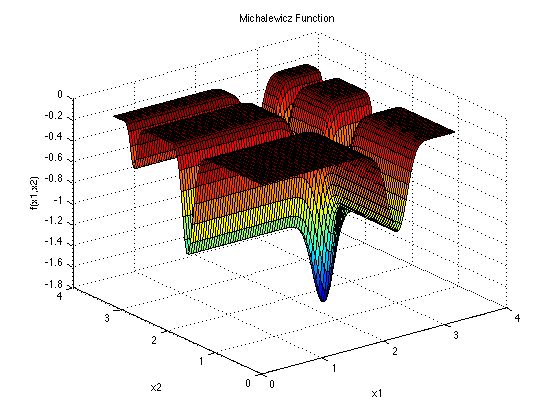
\includegraphics[width=\textwidth,height=\textheight,keepaspectratio]{michal.png}
  \caption{Michalewicz Function\cite{michal_img}}
\end{figure}


\begin{table}[H]
\caption{Values based on 30 runs}
\begin{tblr}{
colspec={X[0.96,l] X[1.7,l] X[1,l] X[1,l] X[1,l] X[1,l]},
rowsep=0.01pt,  % Reduce the vertical padding between cell contents and borders
  cell{1}{1} = {c=2}{},
  cell{2}{1} = {r=4}{c},
  cell{6}{1} = {r=4}{c},
  cell{10}{1} = {r=4}{c},
  vlines,
  hline{1-2,6,10,14} = {-}{},
  hline{3-5,7-9,11-13} = {2-7}{},
}
     &              & HC Best & HC  First & HC Worst & SA Best & GA\\
D = 5 & Mean error & 0.000 & 0.001 & 0.000 & 0.000 & 0.007\\
     &   SDev error & 0.001 & 0.004 & 0.001 & 0.004 & 0.086\\
     &   Min error & 0.000 & 0.000 & 0.000 & 0.000 & 0.000\\
     &   Max error & 0.003 & 0.018 & 0.004 & 0.022 & 0.331\\

D = 10 & Mean error & 0.302 & 0.361 & 0.283 & 0.282 & 0.325\\
     &   SDev error & 0.084 & 0.113 & 0.092 & 0.106 & 0.213\\
     &   Min error & 0.106 & 0.172 & 0.008 & 0.018 & 0.016\\
     &   Max error & 0.452 & 0.598 & 0.407 & 0.459 & 0.884\\

D = 30 & Mean error & 2.693 & 3.227 & 2.764 & 2.845 & 3.675\\
     &   SDev error & 0.223 & 0.258 & 0.253 & 0.296 & 0.692\\
     &   Min error & 2.030 & 2.750 & 2.101 & 1.883 & 2.864\\
     &   Max error & 3.032 & 3.942 & 3.088 & 3.434 & 5.559\\
\end{tblr}
\caption{Hill Climbing time (in seconds) based on 30 runs}
\begin{tblr}{
colspec={X[0.96,l] X[1.7,l] X[1,l] X[1,l] X[1,l] X[1,l]},
rowsep=0.01pt,  % Reduce the vertical padding between cell contents and borders
  cell{1}{1} = {c=2}{},
  cell{2}{1} = {r=4}{c},
  cell{6}{1} = {r=4}{c},
  cell{10}{1} = {r=4}{c},
  vlines,
  hline{1-2,6,10,14} = {-}{},
  hline{3-5,7-9,11-13} = {2-7}{},
}
     &              & HC Best & HC  First & HC Worst & SA Best & GA\\
D = 5 & Mean time & 1.206 & 0.832 & 1.277 & 6.837 & 0.203\\
     &   SDev time & 0.036 & 0.006 & 0.040 & 0.012 & 0.002\\
     &   Min time & 1.147 & 0.820 & 1.211 & 6.803 & 0.196\\
     &   Max time & 1.265 & 0.842 & 1.374 & 6.882 & 0.211\\

D = 10 & Mean time & 10.053 & 5.706 & 8.668 & 25.085 & 0.384\\
     &   SDev time & 0.259 & 0.033 & 0.232 & 0.035 & 0.004\\
     &   Min time & 9.125 & 5.666 & 8.331 & 25.034 & 0.367\\
     &   Max time & 10.440 & 5.849 & 9.313 & 25.203 & 0.399\\

D = 30 & Mean time & 229.089 & 123.951 & 193.611 & 210.705 & 1.067\\
     &   SDev time & 4.395 & 3.759 & 5.031 & 0.898 & 0.010\\
     &   Min time & 225.808 & 113.541 & 187.292 & 208.883 & 1.035\\
     &   Max time & 239.067 & 128.653 & 205.007 & 211.160 & 1.098\\

\end{tblr}
\end{table}
\newpage
\subsection{De Jong Function\cite{dejong}}

$$
f(x) = \sum^n_{i=1}{x_i^2},
x_i \in \left[ -5.12 , 5.12 \right]
$$

The global minima is located at $f(x)=0; x(i)=0,  \forall i=1:n $

\begin{figure}[!h]
  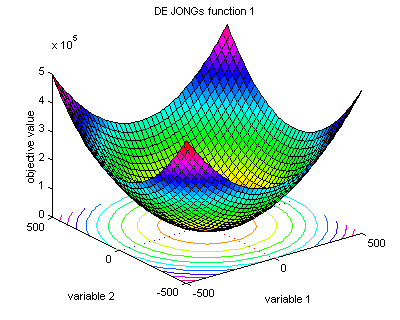
\includegraphics[width=\textwidth,height=\textheight,keepaspectratio]{dejong.png}
  \caption{De Jong Function Function\cite{dejong_img}}
\end{figure}

\begin{table}[H]
\caption{Values based on 30 runs}
\begin{tblr}{
colspec={X[0.96,l] X[1.7,l] X[1,l] X[1,l] X[1,l] X[1,l]},
rowsep=0.01pt,  % Reduce the vertical padding between cell contents and borders
  cell{1}{1} = {c=2}{},
  cell{2}{1} = {r=4}{c},
  cell{6}{1} = {r=4}{c},
  cell{10}{1} = {r=4}{c},
  vlines,
  hline{1-2,6,10,14} = {-}{},
  hline{3-5,7-9,11-13} = {2-7}{},
}
     &              & HC Best & HC  First & HC Worst & SA Best & GA\\
D = 5 & Mean error & 0.000 & 0.000 & 0.000 & 0.000 & 0.000\\
     &   SDev error & 0.000 & 0.000 & 0.000 & 0.000 & 0.000\\
     &   Min error & 0.000 & 0.000 & 0.000 & 0.000 & 0.000\\
     &   Max error & 0.000 & 0.000 & 0.000 & 0.000 & 0.000\\

D = 10 & Mean error & 0.000 & 0.000 & 0.000 & 0.000 & 0.000\\
     &   SDev error & 0.000 & 0.000 & 0.000 & 0.000 & 0.000\\
     &   Min error & 0.000 & 0.000 & 0.000 & 0.000 & 0.000\\
     &   Max error & 0.000 & 0.000 & 0.000 & 0.000 & 0.000\\

D = 30 & Mean error & 0.000 & 0.000 & 0.000 & 0.000 & 0.000\\
     &   SDev error & 0.000 & 0.000 & 0.000 & 0.000 & 0.000\\
     &   Min error & 0.000 & 0.000 & 0.000 & 0.000 & 0.000\\
     &   Max error & 0.000 & 0.000 & 0.000 & 0.000 & 0.000\\
       
\end{tblr}
\caption{Hill Climbing time (in seconds) based on 30 runs}
\begin{tblr}{
colspec={X[0.96,l] X[1.7,l] X[1,l] X[1,l] X[1,l] X[1,l]},
rowsep=0.01pt,  % Reduce the vertical padding between cell contents and borders
  cell{1}{1} = {c=2}{},
  cell{2}{1} = {r=4}{c},
  cell{6}{1} = {r=4}{c},
  cell{10}{1} = {r=4}{c},
  vlines,
  hline{1-2,6,10,14} = {-}{},
  hline{3-5,7-9,11-13} = {2-7}{},
}
     &              & HC Best & HC  First & HC Worst & SA Best & GA\\
D = 5 & Mean time & 0.595 & 0.369 & 0.557 & 3.449 & 0.192\\
     &   SDev time & 0.010 & 0.002 & 0.005 & 0.013 & 0.001\\
     &   Min time & 0.584 & 0.363 & 0.553 & 3.435 & 0.192\\
     &   Max time & 0.617 & 0.371 & 0.585 & 3.474 & 0.198\\

D = 10 & Mean time & 4.671 & 2.407 & 3.812 & 10.824 & 0.337\\
     &   SDev time & 0.210 & 0.017 & 0.029 & 0.075 & 0.005\\
     &   Min time & 4.216 & 2.387 & 3.755 & 10.649 & 0.336\\
     &   Max time & 4.912 & 2.467 & 3.912 & 10.925 & 0.369\\

D = 30 & Mean time & 106.610 & 53.719 & 85.543 & 76.099 & 0.961\\
     &   SDev time & 1.254 & 0.544 & 0.612 & 0.811 & 0.007\\
     &   Min time & 102.922 & 52.773 & 84.489 & 75.731 & 0.941\\
     &   Max time & 107.812 & 54.546& 87.371 & 79.257 & 0.973\\
\end{tblr}
\end{table}
\newpage
\subsection{Schwefel Function\cite{schwef}}

$$
f(x) = 418.982n - \sum_{i=1}^n{x_i\sin(\sqrt{\left|x_i\right|})},
x_i \in \left[ -500 , 500 \right]
$$

The global minima is located at $f(x)=0; x(i)=0,  \forall i=1:n $

\begin{figure}[!h]
  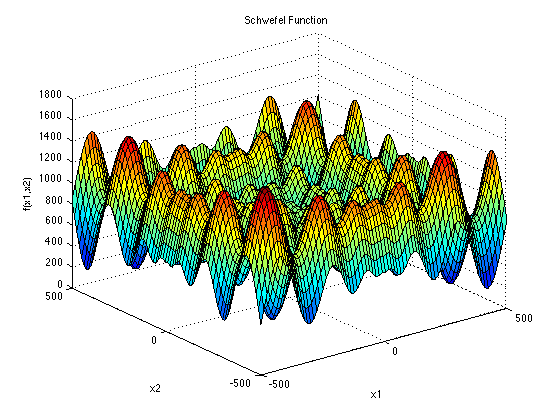
\includegraphics[width=\textwidth,height=\textheight,keepaspectratio]{schwef.png}
  \caption{Schwefel Function\cite{schwef_img}}
\end{figure}

\begin{table}[H]
\caption{Values based on 30 runs}
\begin{tblr}{
colspec={X[0.96,l] X[1.7,l] X[1,l] X[1,l] X[1,l] X[1,l]},
rowsep=0.01pt,  % Reduce the vertical padding between cell contents and borders
  cell{1}{1} = {c=2}{},
  cell{2}{1} = {r=4}{c},
  cell{6}{1} = {r=4}{c},
  cell{10}{1} = {r=4}{c},
  vlines,
  hline{1-2,6,10,14} = {-}{},
  hline{3-5,7-9,11-13} = {2-7}{},
}
     &              & HC Best & HC  First & HC Worst & SA Best & GA\\
D = 5 & Mean error & 0.104 & 34.236 & 0.104 & 0.104 & 0.177\\
     &   SDev error & 0.091 & 28.681 & 0.072 & 0.094 & 0.131\\
     &   Min error & 0.000 & 0.001 & 0.000 & 0.000 & 0.002\\
     &   Max error & 0.311 & 118.542 & 0.208 & 0.312 & 0.439\\

D = 10 & Mean error & 119.151 & 305.854 & 119.360 & 152.937 & 30.249\\
     &   SDev error & 55.845 & 75.565 & 62.588 & 51.430 & 59.370\\
     &   Min error & 0.520 & 119.344 & 0.519 & 34.547 & 0.486\\
     &   Max error & 187.329 & 424.103 & 199.698 & 234.581 & 273.941\\

D = 30 & Mean error & 1221.768 & 1812.850 & 1238.527 & 1243.475 & 845.000\\
     &   SDev error & 141.610 & 154.695 & 134.361 & 157.466 & 291.677\\
     &   Min error & 789.557 & 1383.452 & 893.080 & 805.879 & 455.446\\
     &   Max error & 1407.216 & 2016.318 & 1462.854 & 1463.694 & 1952.879\\
\end{tblr}
\caption{Hill Climbing time (in seconds) based on 30 runs}
\begin{tblr}{
colspec={X[0.96,l] X[1.7,l] X[1,l] X[1,l] X[1,l] X[1,l]},
rowsep=0.01pt,  % Reduce the vertical padding between cell contents and borders
  cell{1}{1} = {c=2}{},
  cell{2}{1} = {r=4}{c},
  cell{6}{1} = {r=4}{c},
  cell{10}{1} = {r=4}{c},
  vlines,
  hline{1-2,6,10,14} = {-}{},
  hline{3-5,7-9,11-13} = {2-7}{},
}
     &              & HC Best & HC  First & HC Worst & SA Best & GA\\
D = 5 & Mean time & 1.731 & 1.062 & 1.639 & 6.772 & 0.260\\
     &   SDev time & 0.336 & 0.007 & 0.007 & 0.026 & 0.011\\
     &   Min time & 1.630 & 1.053 & 1.630 & 6.713 & 0.249\\
     &   Max time & 2.725 & 1.095 & 1.668 & 6.797 & 0.299\\

D = 10 & Mean time & 14.024 & 7.342 & 11.386 & 22.644 & 0.476\\
     &   SDev time & 0.265 & 0.111 & 0.042 & 0.029 & 0.017\\
     &   Min time & 12.919 & 6.832 & 11.298  & 22.583 & 0.460\\
     &   Max time & 14.511 & 7.375 & 11.478& 22.704 & 0.524\\

D = 30 & Mean time & 334.324 & 160.868 & 278.862 & 171.217 & 1.353\\
     &   SDev time & 9.762 & 0.915 & 0.900 & 3.060 & 0.052\\
     &   Min time & 319.042 & 160.159 & 276.551 & 168.317 & 1.303\\
     &   Max time & 349.083 & 164.243 & 280.273 & 176.714 & 1.511\\
\end{tblr}
\end{table}


\section{Comparing Methods}
Comparing the Genetic Algorithm (GA) to Hill Climbing methods, we observed that the GA is significantly faster but may not always find the most accurate solution. Specifically, our experiments show that the GA is, on average, 6653\% faster but 8\% less correct compared to the Hill Climbing algorithm.

\section{Conclusions}
The Genetic Algorithm is effective for optimizing mathematical functions, offering a significant speed advantage over Hill Climbing methods. However, its performance in terms of accuracy can be slightly lower. Hill Climbing algorithms can provide more accurate solutions but at the cost of increased computational time. In the future, it would be interesting to explore using a meta-genetic algorithm to tune parameters, such as deciding when to switch to Gray encoding for the last 10\% of generations or for the entire run.


\begin{thebibliography}{9}

\bibitem{rast_img}
Authors: Sonja Surjanovic \& Derek Bingham, Simon Fraser University \\ Rastrigin's Function rendered image.
  \url{https://www.sfu.ca/~ssurjano/rastr.html}

\bibitem{Rastrigin}
  Rastrigin, L. A. "Systems of extremal control." Mir, Moscow (1974).

\bibitem{michal_img}
Authors: Sonja Surjanovic \& Derek Bingham, Simon Fraser University \\ Michalewicz's Function rendered image.
  \url{https://www.sfu.ca/~ssurjano/michal.html}

\bibitem{michal}
    Michalewicz, Zbigniew. "A survey of constraint handling techniques in evolutionary computation methods." (1995).

\bibitem{dejong_img}
Dejong's Function rendered image.
  \url{http://www.geatbx.com/docu/fcnindex-msh_f1_500-2.gif}

\bibitem{dejong}
De Jong, Kenneth Alan. An analysis of the behavior of a class of genetic adaptive systems. University of Michigan, 1975.

\bibitem{schwef_img}
Authors: Sonja Surjanovic \& Derek Bingham, Simon Fraser University \\ Schwefel's Function rendered image.
  \url{https://www.sfu.ca/~ssurjano/schwef.html}

\bibitem{schwef}
Bäck, Thomas, and Hans-Paul Schwefel. "An overview of evolutionary algorithms for parameter optimization." Evolutionary computation 1.1 (1993): 1-23.

\bibitem{glob_min}
Vanaret, Charlie, et al. "Certified global minima for a benchmark of difficult optimization problems." arXiv preprint arXiv:2003.09867(2020).


\end{thebibliography} 


\end{document}




